\documentclass[12pt,tikz]{standalone}
\pdfinfoomitdate 1
\pdfsuppressptexinfo 1
\pdftrailerid{}
\usepackage[utf8]{inputenc}
\usepackage{amsmath}
\usepackage{pgfplots}
\usepackage{tikz}
\usetikzlibrary{shapes.geometric}
\pagestyle{empty}

\begin{document}
\begin{tikzpicture}
	\tikzstyle{process} = [draw, fill=green!10, rectangle, minimum height=3em, minimum width=10em, node distance=5em, font={\ttfamily}]
	\tikzstyle{data} = [draw, fill=blue!10, ellipse, minimum height=3em, minimum width=7em, node distance=5em, font={\ttfamily}]

	\node[data]    (n1)               {Verilog Source};
	\node[process] (n2) [below of=n1] {Verilog Frontend};
	\node[data]    (n3) [below of=n2] {AST};
	\node[process] (n4) [below of=n3] {AST Frontend};
	\node[data]    (n5) [below of=n4] {RTLIL};

	\draw[-latex] (n1) -- (n2);
	\draw[-latex] (n2) -- (n3);
	\draw[-latex] (n3) -- (n4);
	\draw[-latex] (n4) -- (n5);

	\tikzstyle{details} = [draw, fill=yellow!5, rectangle, node distance=6cm, font={\ttfamily}]

	\node[details] (d1) [right of=n2] {\begin{minipage}{5cm}
		\hfil
		\begin{tikzpicture}
			\tikzstyle{subproc} = [draw, fill=green!10, rectangle, minimum height=2em, minimum width=10em, node distance=3em, font={\ttfamily}]
			\node (s0) {};
			\node[subproc] (s1) [below of=s0] {Preprocessor};
			\node[subproc] (s2) [below of=s1] {Lexer};
			\node[subproc] (s3) [below of=s2] {Parser};
			\node[node distance=3em] (s4) [below of=s3] {};
			\draw[-latex] (s0) -- (s1);
			\draw[-latex] (s1) -- (s2);
			\draw[-latex] (s2) -- (s3);
			\draw[-latex] (s3) -- (s4);
		\end{tikzpicture}
	\end{minipage}};

	\draw[dashed] (n2.north east) -- (d1.north west);
	\draw[dashed] (n2.south east) -- (d1.south west);

	\node[details] (d2) [right of=n4] {\begin{minipage}{5cm}
		\hfil
		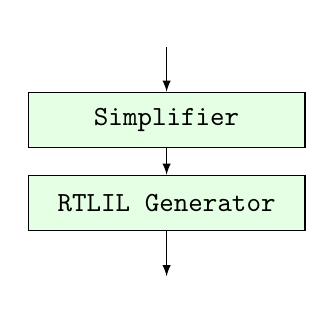
\begin{tikzpicture}
			\tikzstyle{subproc} = [draw, fill=green!10, rectangle, minimum height=2em, minimum width=10em, node distance=3em, font={\ttfamily}]
			\node (s0) {};
			\node[subproc] (s1) [below of=s0] {Simplifier};
			\node[subproc] (s2) [below of=s1] {RTLIL Generator};
			\node[node distance=3em] (s3) [below of=s2] {};
			\draw[-latex] (s0) -- (s1);
			\draw[-latex] (s1) -- (s2);
			\draw[-latex] (s2) -- (s3);
		\end{tikzpicture}
	\end{minipage}};

	\draw[dashed] (n4.north east) -- (d2.north west);
	\draw[dashed] (n4.south east) -- (d2.south west);

\end{tikzpicture}
\end{document}
